\documentclass[herrin-thesis.tex]{subfiles}
\begin{document}

\section{Electron Capture on Impurities}
When an electromagnetic process deposits energy in a nobel liquid detector, it ionizes the atoms, producing electrons and ions. Some of the electrons will recombine with the ions, which produces scintillation light. However, if the detector has an applied electric field, then the remaining electrons and ions will drift in opposite directions along the field lines. In a detector consisting of perfectly pure nobel liquid, the electrons would all reach the anode and would be collected for an energy measurement. In a non-ideal detector, however, electronegative impurities can capture the drifting electrons and form ions. The ions are more massive and drift more slowly, and so they escape inclusion in the signal used for energy measurement.

Electronegative impurities may capture electrons in three ways\cite{Aprile:2006fk}. I denote the impurities, which may be atoms or molecules, as \(AB\):
\begin{enumerate}
\item Radiative attachment
\begin{equation}
e^{-} + AB \rightarrow AB^{-} + h \nu
\end{equation}
which has a much smaller cross section than the other processes below.
\item Dissociative attachment
\begin{equation}
\begin{split}
e^{-} + AB \rightarrow e^{-} + AB^{*} \rightarrow A^{+} + B^{-} + e^{-} \\
e^{-} + AB \rightarrow AB^{-} \rightarrow A^{+} + B^{-}
\end{split}
\end{equation}
which requires the electron's energy to be much higher than typically found for an electron drifting in a liquid or dense gas.
\item Three-body attachment through the two-stage Bloch-Bradbury reaction
\begin{equation}
\begin{split}
e^{-} + AB \leftrightarrow (AB^{-})^{*} \\
(AB^{-})^{*} + X \rightarrow AB^{-} + X
\end{split}
\label{eq:3bodyattachment}
\end{equation}
where X represents the atom or molecule that make up the majority of the liquid.
\end{enumerate}

The three-body reaction shown in \cref{eq:3bodyattachment} releases some amount of energy, given by the \emph{electron affinity} of \(AB\). The electron affinity is positive if \(AB\) is electronegative. Nobel elements have a negative electron affinity, so the reaction does not take place in a pure detector.

The rate of the reaction shown in \cref{eq:3bodyattachment} is given by:
\begin{equation}
\frac{dn_{AB}}{dt} = -k_{3} n_{AB} n_{X} n_{e^{-}}
\label{eq:3bodyreactionrate}
\end{equation}
where \(k_3\) is constant for the 3-body reaction, and \(n_{AB}\), \(n_{X}\), and \(n_{e^{-}}\) are the densities of the impurity, the atoms or molecules of the liquid, and the electrons, respectively. \(k_3\) depends on the species of the impurity, the species of the liquid, and the electric field strength.

According to \cref{eq:3bodyreactionrate}, electrons will be captured, forming \(AB^{-}\) at a rate proportional to the density of electrons. Thus, the number of free electrons will decay exponentially over time according to:
\begin{equation}
N_{e^{-}}(t) = N_0 \exp (-t/\tau_e)
\label{eq:exponentialtaue}
\end{equation}
where \(N_0\) is the original number of electrons, and \(\tau_e\) is the \emph{electron lifetime}.

In general, there can be several different species of electronegative impurity. In that case, they all contribute to the electron lifetime according to:
\begin{equation}
\tau_e^{-1} = \sum_i k_i n_i = \sum_i\tau_i^{-1}
\label{eq:tauedefinition}
\end{equation}
where \(n_i\) is the density of an electronegative impurity and \(k_i\) is the cross section for electron capture by that impurity. For most impurities, \(k_i\) depends on the electric field strength.

\section{Measuring Electron Lifetime}

\subsection{Method}
\Cref{eq:exponentialtaue} provides a simple recipe for measuring the electron lifetime: measure the exponential attenuation of a known quantity of ionization as a function of drift time. All full absorption peaks from gamma-ray lines will create roughly the same amount of ionization, following a Gaussian distribution with its width provided by the Fano factor and detector resolution. If some of the ionization is being attenuated, then the peak's mean will shift downward in energy from its true value.

A single calibration source at the cathode of the detector produces illuminates both TPCs, and the gamma rays interact throughout the entire drift region. After a sufficiently long calibration run, I divide the TPC into drift time bins. The size of the bins is a compromise: a larger bin in drift time will have more events, and thus the measurement of the full absorption peak energy will be better. A smaller bin will have fewer events, but will suffer energy smearing since events in the bin that drift farther will be attenuated less. In practice, 16 \todo{Check this} bins seems a good compromise.

In addition to the full-absorption peak, which is Gaussian, the energy spectrum from a gamma ray source will contain a Compton shoulder. That is, some gamma rays will interact without depositing their full energy, and then scatter out of the detector. A simple model for this shoulder is a step function convolved with a Gaussian smearing representing the effects of energy resolution, producing a complementary error function. For each drift time bin, I fit this simple Gaussian + complementary error function model to the energy spectrum of that bin using an unbinned maximum likelihood fit. \Cref{fig:dtbinfit} shows an example fit.

\begin{figure}[htbp]
\centering
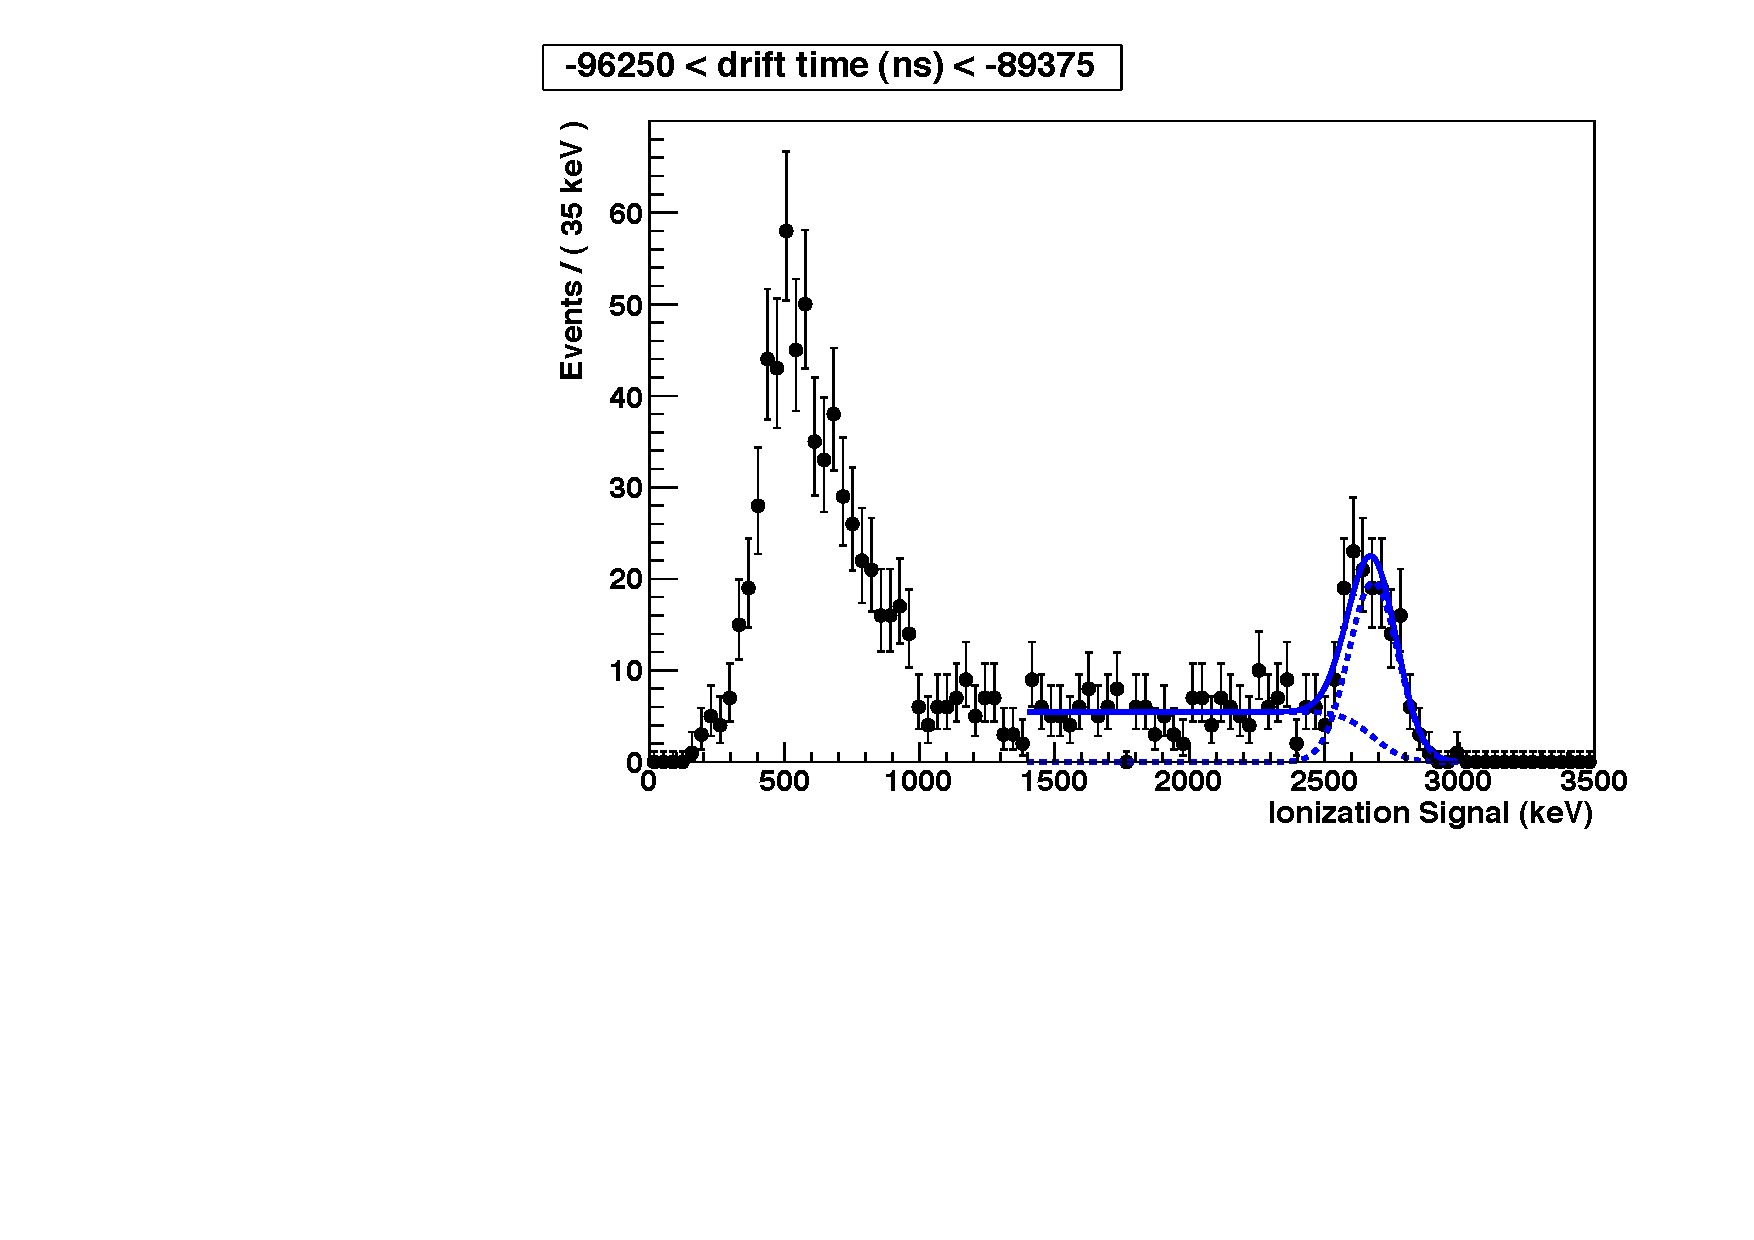
\includegraphics[width=0.8\columnwidth]{./plots/el_run4034_dt_bin_fit.pdf}
\caption[An example fit in a drift time bin]{A fit of the simple Gaussian + complementary error function model to one single drift time bin. In this example, the full absorption peak is the 2615 keV gamma line from \thorium{228}.}
\label{fig:dtbinfit}
\end{figure}

Plotting the full absorption peak energy from each drift time bin as a function of drift time reveals the exponential decay described in \cref{eq:exponentialtaue}. Fitting an exponential to each TPC yields a measurement of the electron lifetime for each. Alternatively, a fit with a single electron lifetime to the entire detector uses information from both TPCs. In all cases, the amplitude of the exponential is allowed to float in the fit, since only the relative decay matters when measuring the electron lifetime. Presently, the separate TPC lifetimes are used when correcting for electron lifetime in EXO-200, while the single measurement is used when monitoring the detector and data quality. \Cref{fig:elfit} shows an example.

\begin{figure}[htbp]
\centering
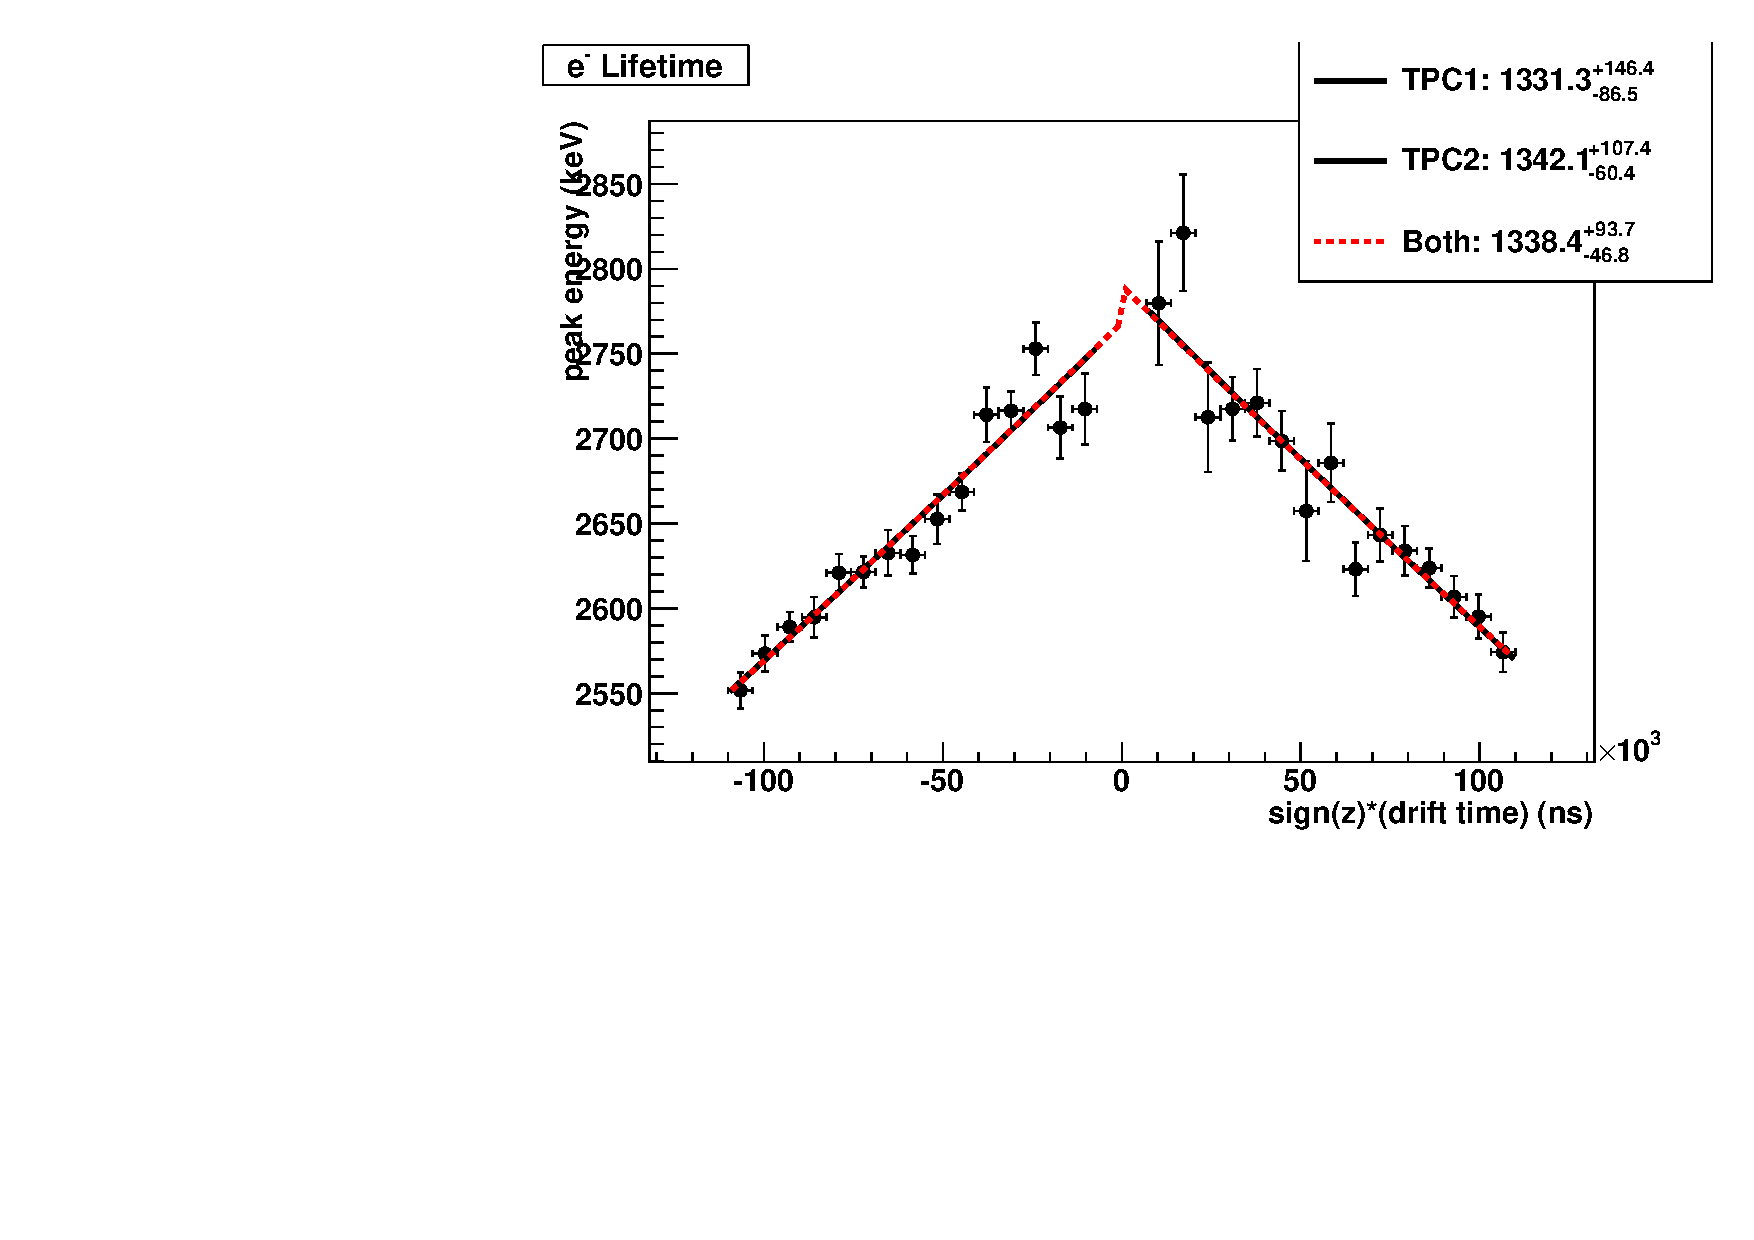
\includegraphics[width=0.8\columnwidth]{./plots/el_run4228_fit.pdf}
\caption[An example fit to exponential attenuation]{Measuring the electron lifetime by fitting a decaying exponential to the full-absorption peak energies binned by drift time. TPC 2 is assigned a negative drift time for convenience in visualization. Both fits to the individual TPCs and to both TPCs together are shown.}
\label{fig:elfit}
\end{figure}

The electron lifetime measurement comes from minimizing the \(\chi^2\) statistic. Confidence intervals for the measurement come from doing a profile scan. That is, the electron lifetime is set to some fixed value away from the best fix, and the amplitude is allowed to vary to minimize \(\chi^2\). All values for which \(\chi^2\) is less than 1 above the minimum value define the 1\(\sigma\) (68\%) confidence band. \Cref{fig:profileel} shows an example.

\begin{figure}[htbp]
\centering
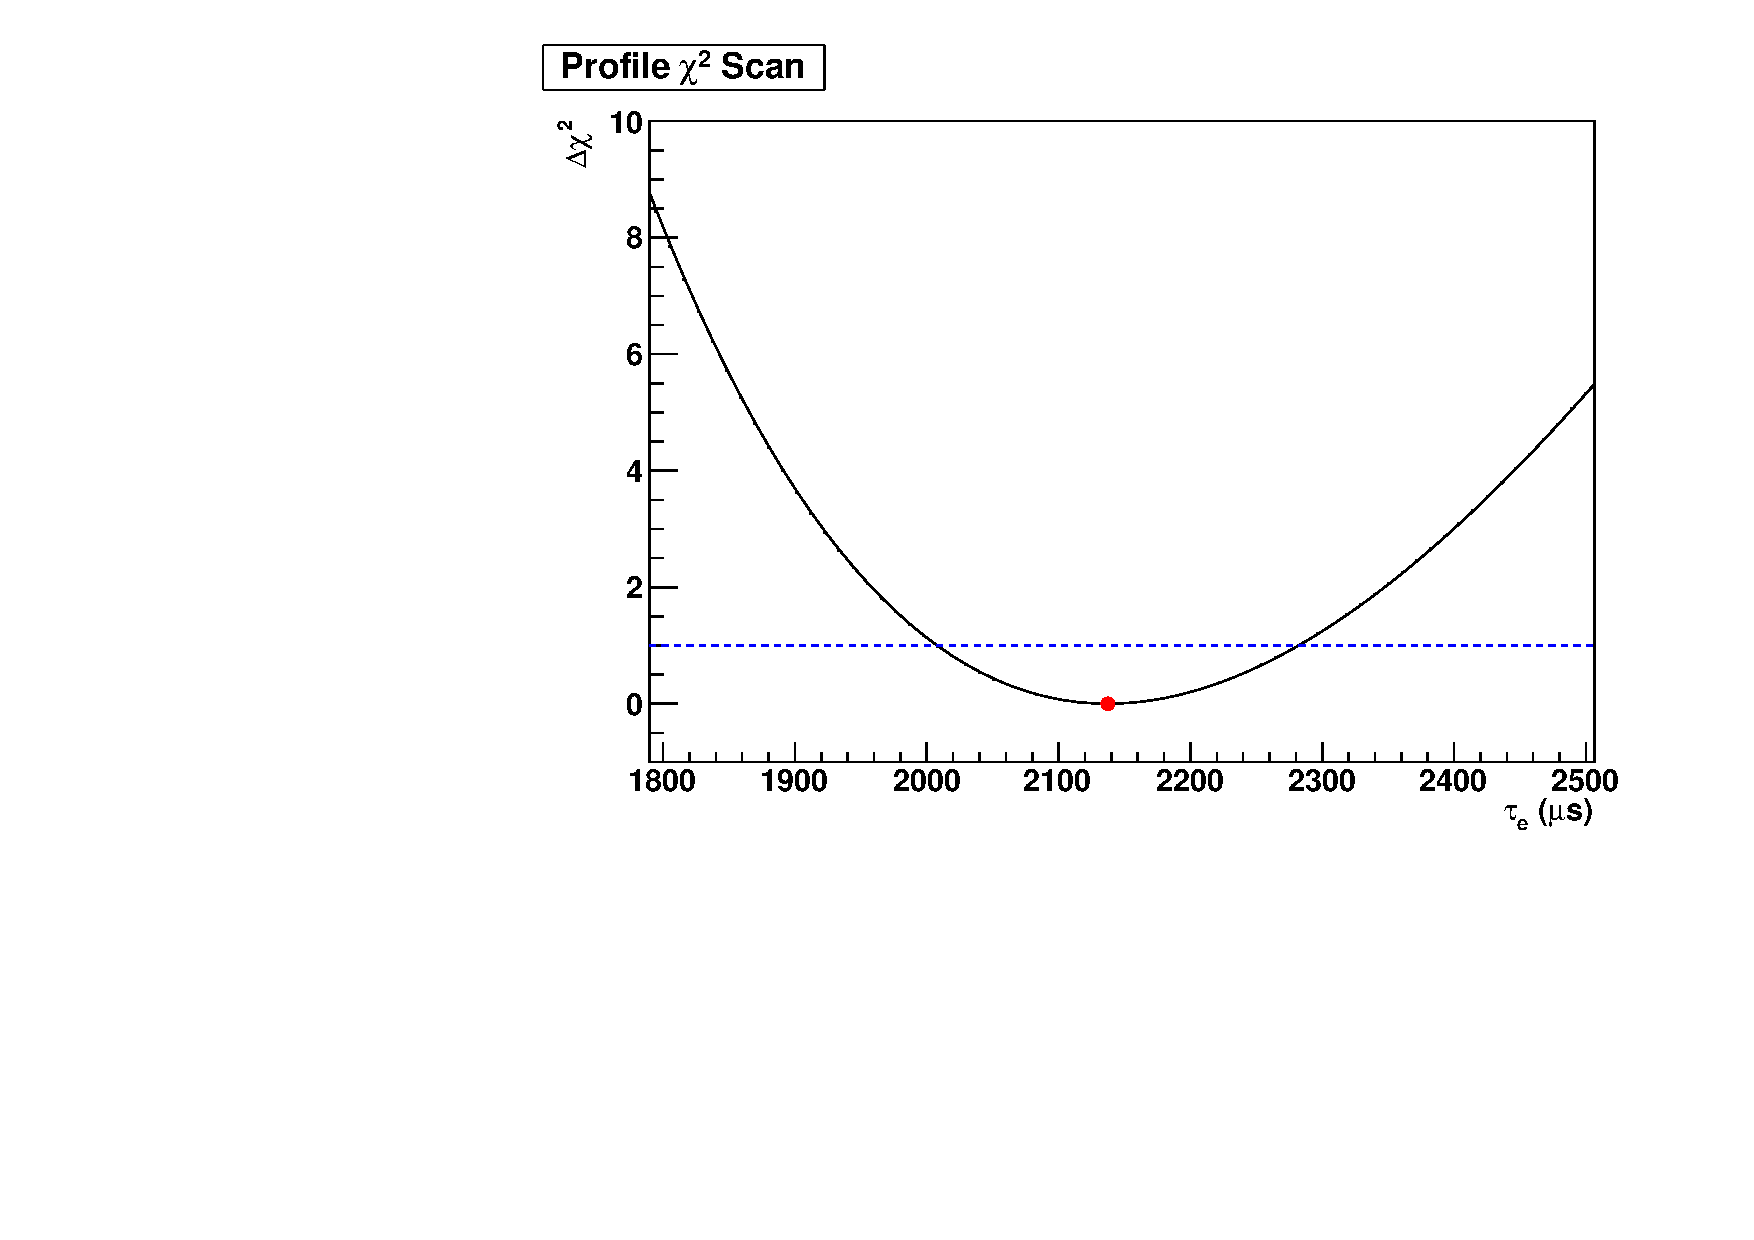
\includegraphics[width=0.8\columnwidth]{./plots/el_run4252_profile.pdf}
\caption[A profile scan around the best-fit electron lifetime]{Confidence intervals around the best fit electron lifetime come from a profile scan, shown here. As this figure shows, this is superior to simply estimating the 1\(\sigma\) errors from the second derivative at the best fit value, since the profile is asymmetric around the best fit (indicated by the red dot). The blue line indicates \(\Delta\chi^2 = 1\), corresponding to a 68\% confidence interval.}
\label{fig:profileel}
\end{figure}

\subsection{Comparison to Simulation}

\Cref{fig:sim_err} shows a comparison between a known simulated electron lifetime and the measurement of that lifetime using the method described above. The method consistently underestimates the electron lifetime, with the effect getting worse as the electron lifetime improves. This could be due to numerical precision issues in the simulation\todo{Actually figure this out.}, or due to the finite width bins used in the fit. The attenuation will not be symmetric around the centers of the bins, and so this could affect the exponential fit.

\begin{figure}[htbp]
\begin{subfigure}[b]{0.5\linewidth}
\centering
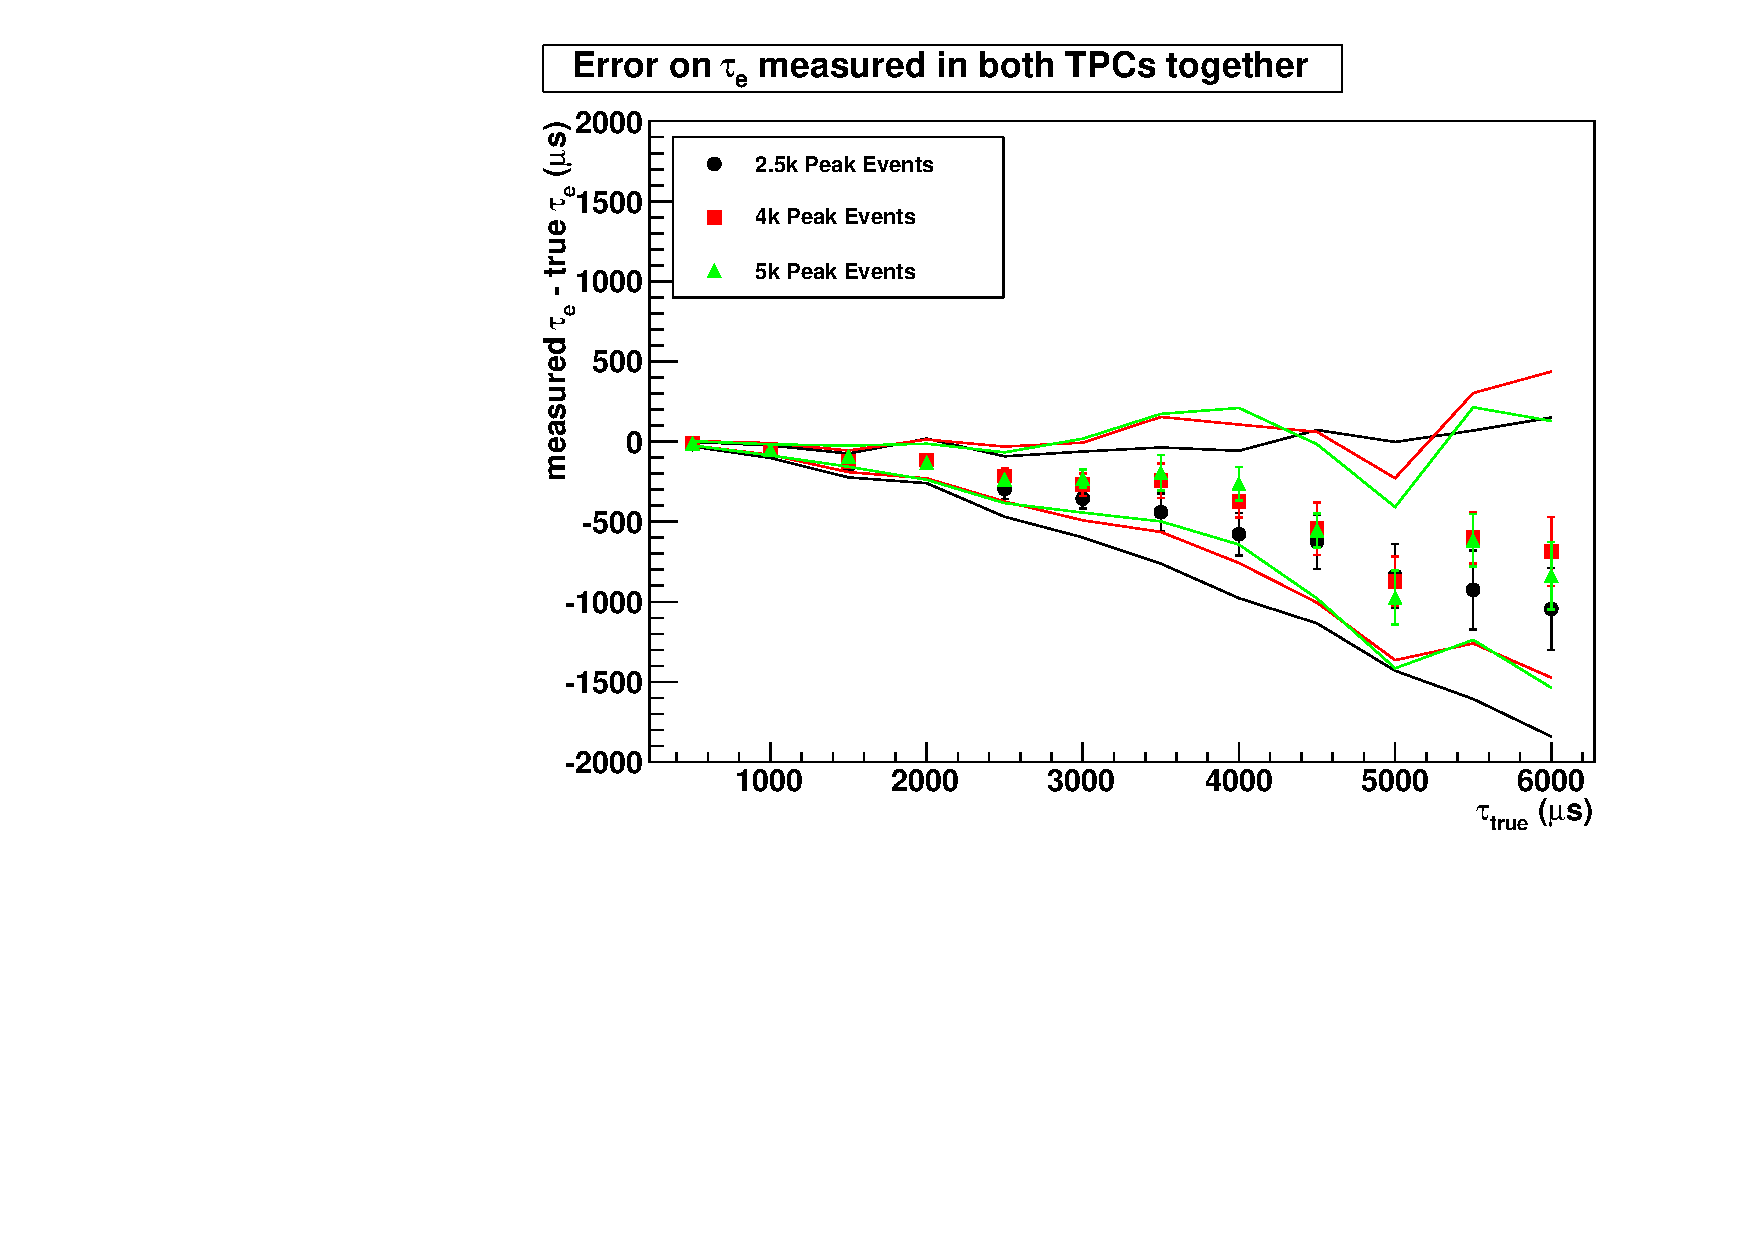
\includegraphics[width=1.0\columnwidth]{./plots/el_sim_error_both.pdf}
\end{subfigure}%
\begin{subfigure}[b]{0.5\linewidth}
\centering
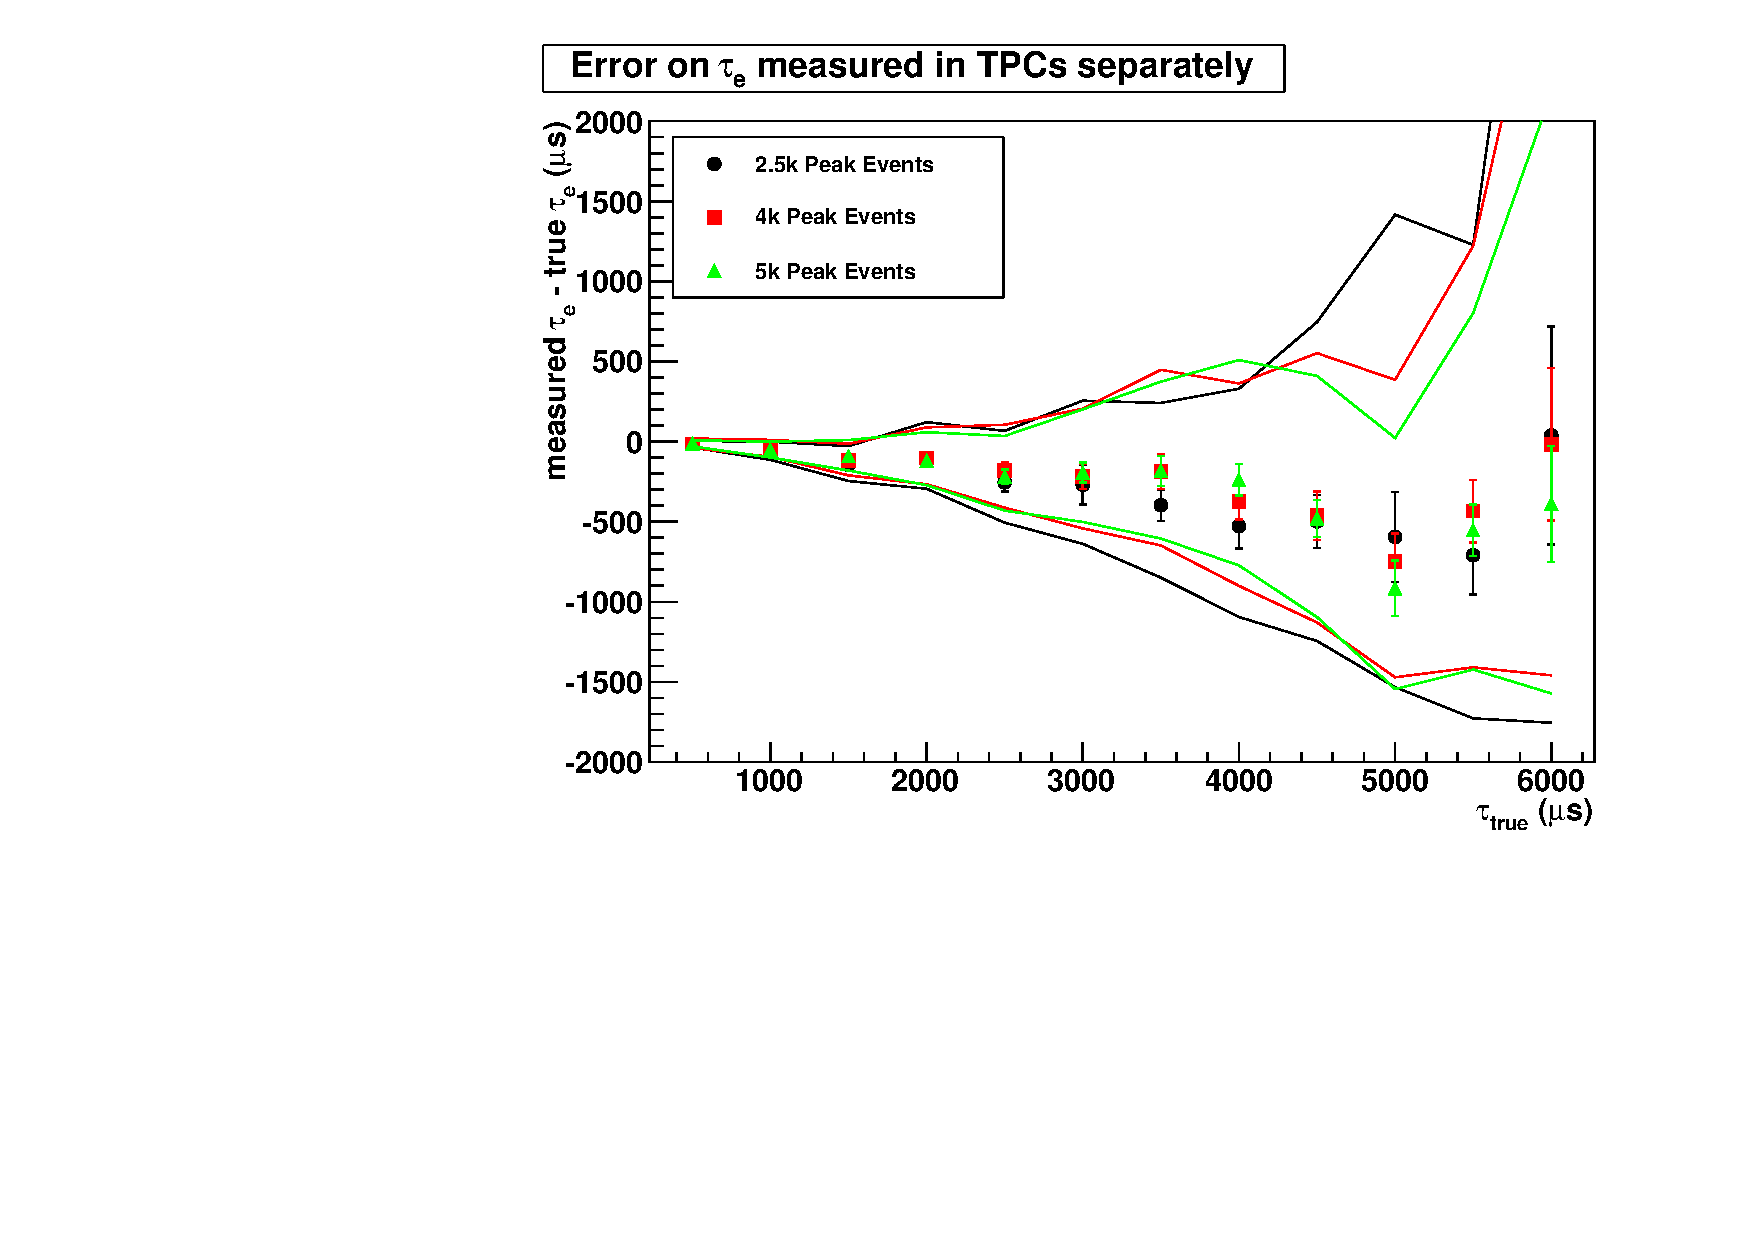
\includegraphics[width=1.0\columnwidth]{./plots/el_sim_error_indiv.pdf}
\end{subfigure}
\caption[Error on reconstructed electron lifetime from simulation]{The absolute error on the electron lifetime measurement for the electron lifetime measured in both TPCs simultaneously (left) and individually (right). The points show the mean error of 20 simulations, and the lines show the mean error on the edges of the 68\% confidence bands for those simulations. The measurement method consistently underestimates the purity, and the error grows as the electron lifetime gets large. Typical calibration runs include 2.5k events in the full absorption peak (black), but using more events would improve the error.}
\label{fig:sim_err}
\end{figure}

This error, if real, is small however. For \SI{3000}{\micro\second} electron lifetime, an applied correction of  \SI{2500}{\micro\second} will only move the measured ionization signal 0.76\% lower than its true value, if the ionization drifts over the full  \SI{120}{\micro\second}  drift time. The effect on the energy resolution will be half this, and will be only a small component of the measured 1.68\% energy resolution \todo{Update this} near the \zeronu region of interest. Furthermore, the error seems to have a simple linear or quadratic dependence on electron lifetime, and so this can be corrected for.\todo{Update when this correction is done, or explain why not.}

\subsection{Practical Considerations}

\begin{figure}[htbp]
\begin{subfigure}[b]{0.5\linewidth}
\centering
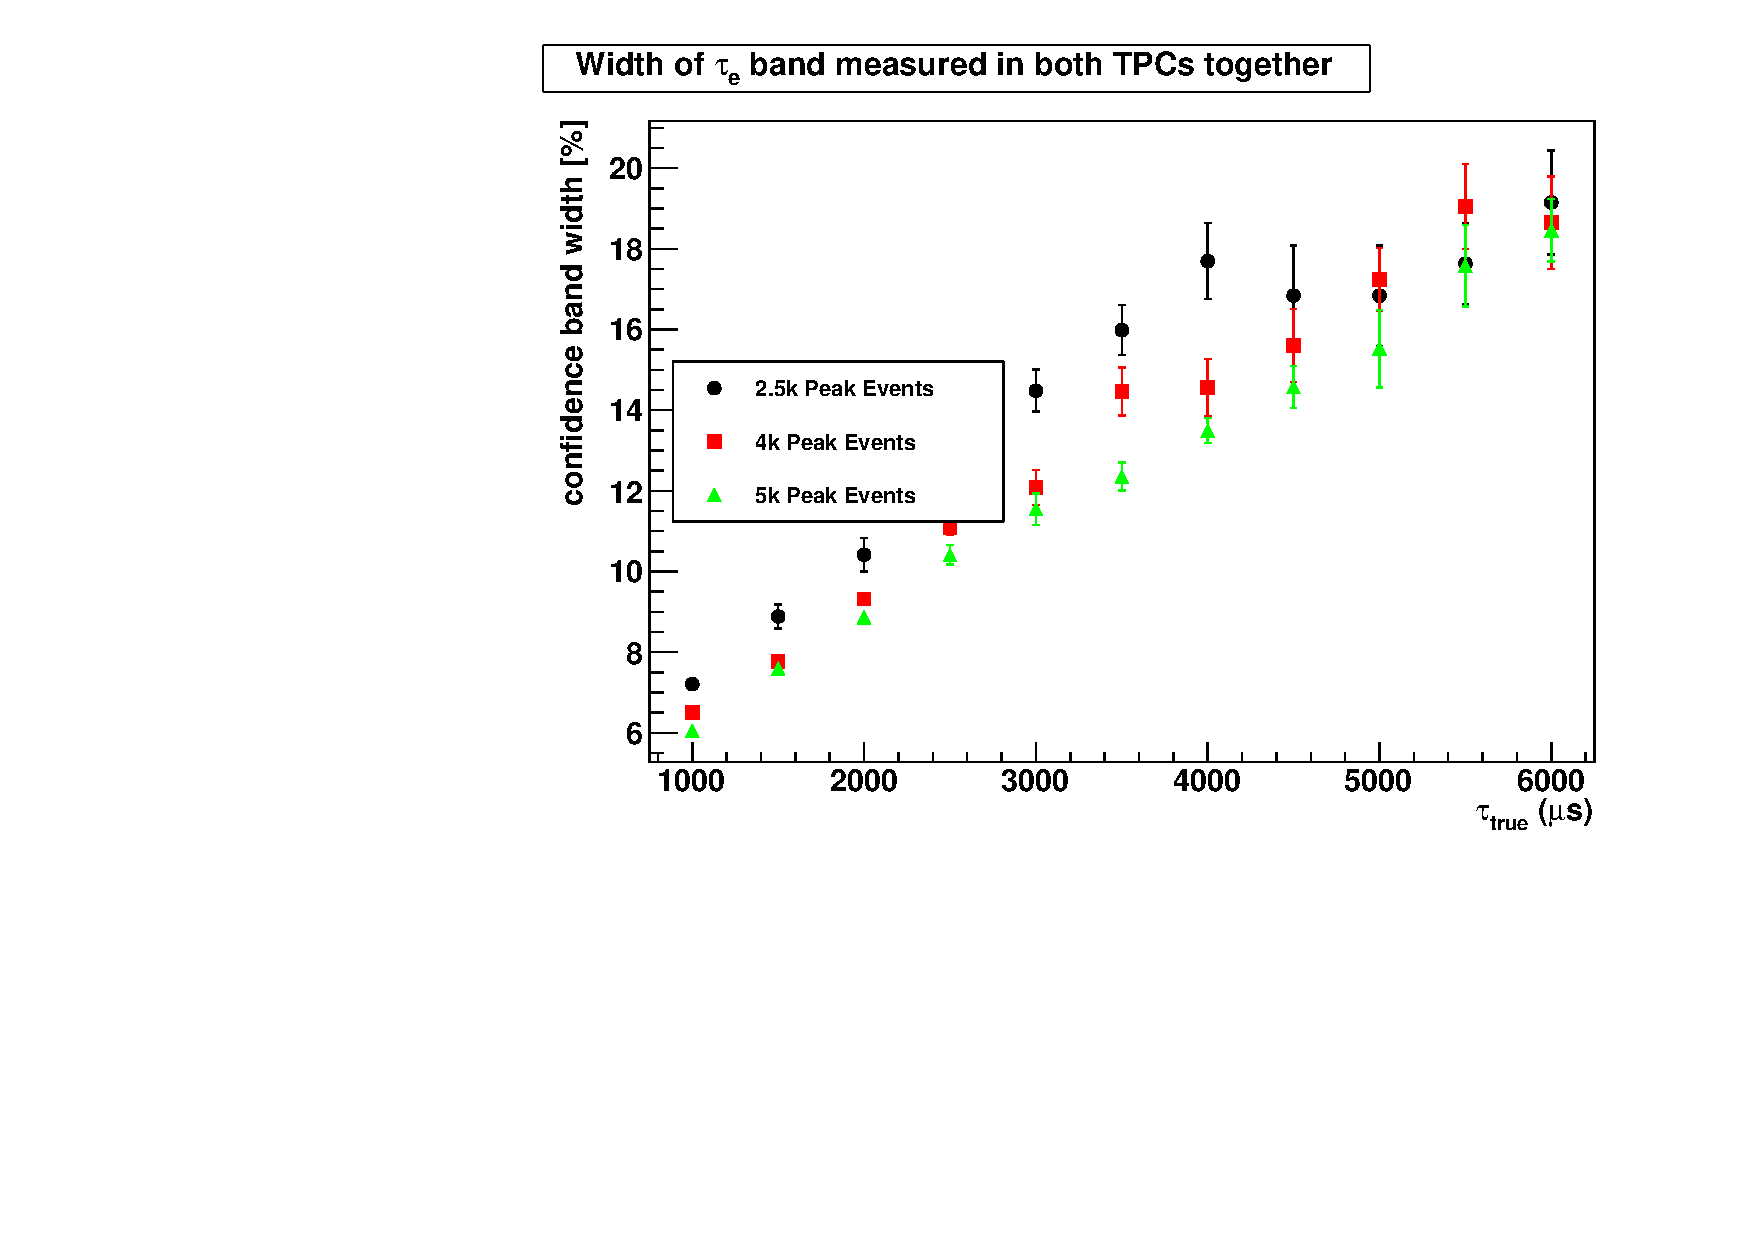
\includegraphics[width=1.0\columnwidth]{./plots/el_sim_width_both.pdf}
\end{subfigure}%
\begin{subfigure}[b]{0.5\linewidth}
\centering
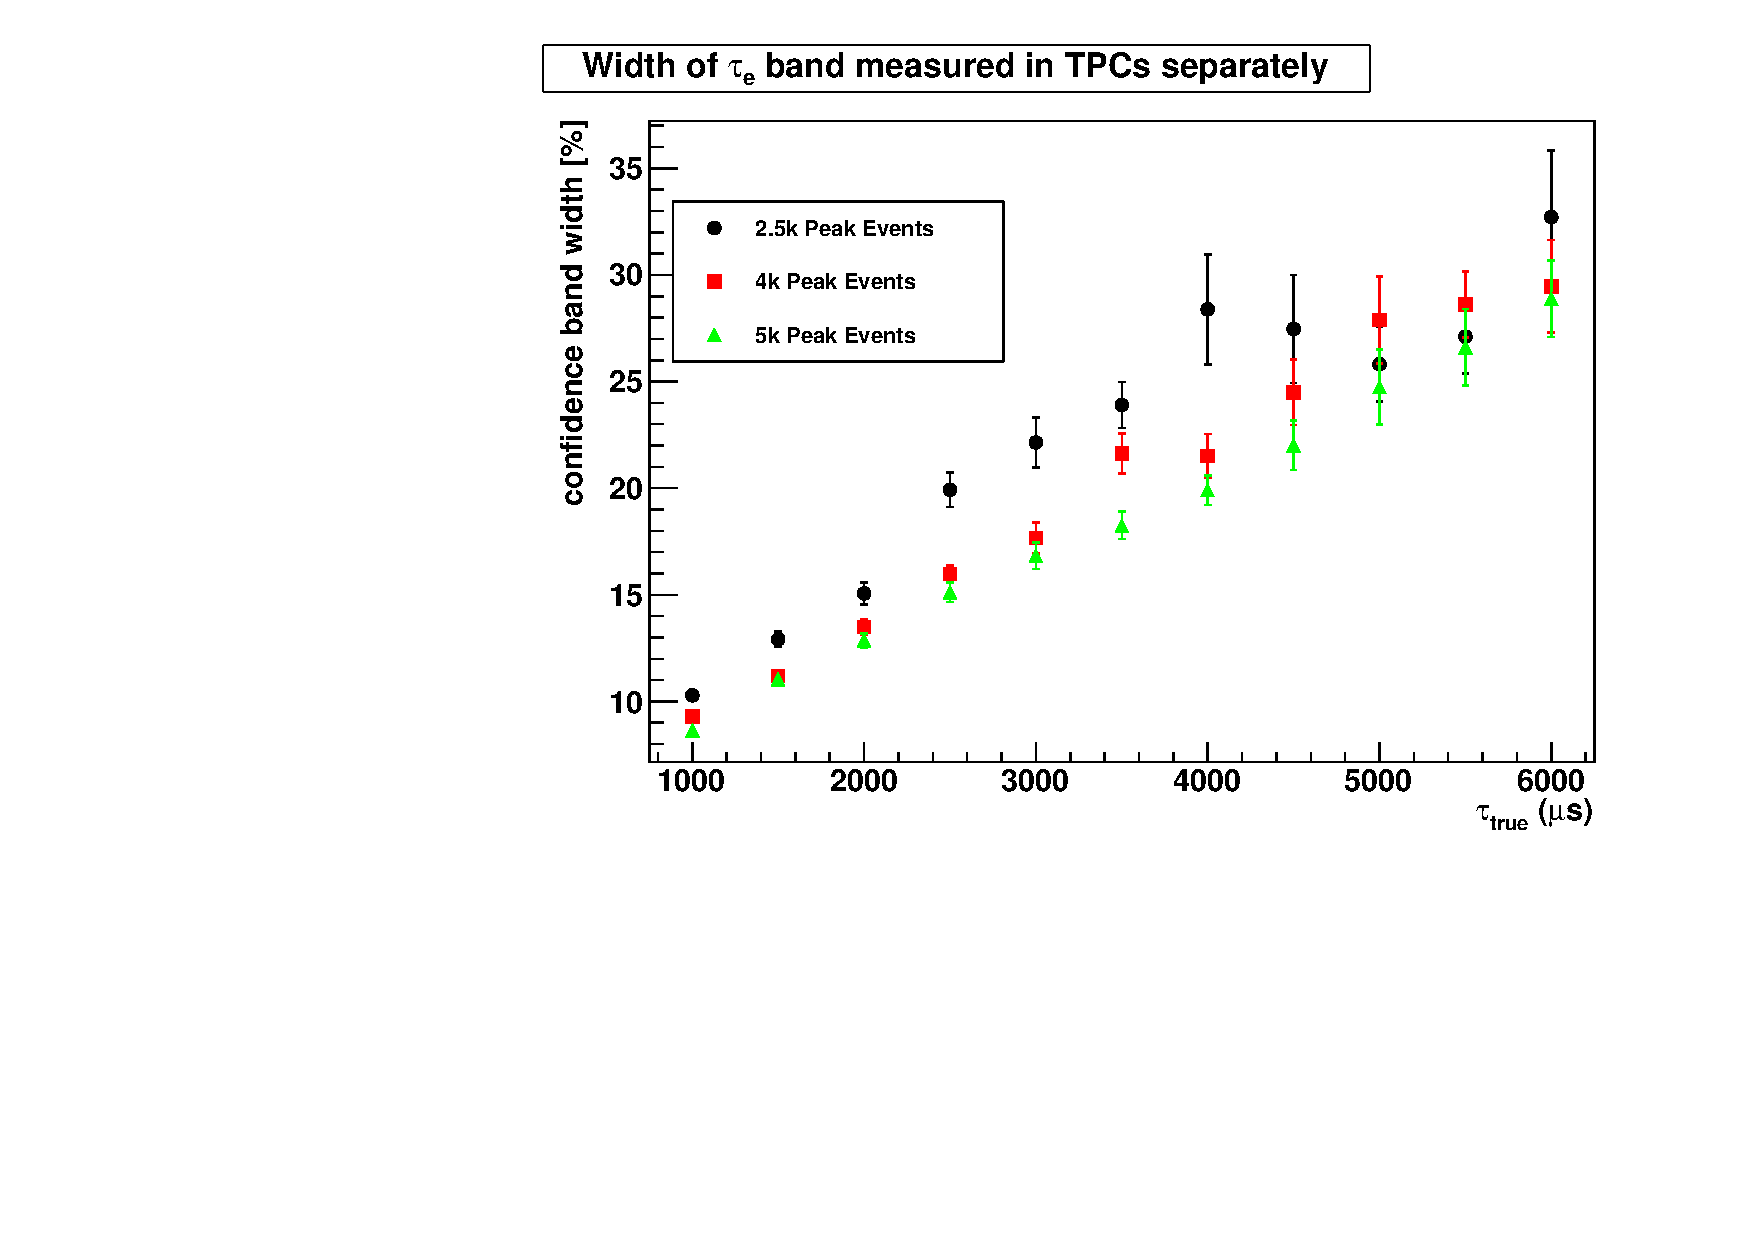
\includegraphics[width=1.0\columnwidth]{./plots/el_sim_width_indiv.pdf}
\end{subfigure}
\caption[Confidence band widths for electron lifetime measurements]{The width of the 68\% confidence band for the electron lifetime measured in both TPCs simultaneously (left) and individually (right). Typical calibration runs include 2.5k events in the full absorption peak (black dots), but using more events would improve the error. Using longer calibrations would improve the uncertainty. However, for long electron lifetimes, it becomes difficult to detect the attenuation and measure it, giving a large uncertainty.}
\label{fig:sim_width}
\end{figure}

As the electron lifetime grows large, it becomes increasingly difficult to measure. For a  \SI{4000}{\micro\second}  electron lifetime, ionization drifting the full distance will only be attenuated about 3\%. This is comparable to the 3.4\% energy resolution in the ionization channel at the 2615 keV full absorption peak from \thorium{228}. This effect is shown in \cref{fig:sim_width}. The width of the confidence band for the measurement grows to near 20\% of the measured value for large electron lifetimes. Taking more calibration data only partially mitigates this effect, also shown in \cref{fig:sim_width}. A simulated calibration run with twice as many events in the photopeak (and requiring twice as much time to run) only shrinks the confidence band by roughly \(\sqrt{2}\).

\subsection{Effects of Electron Lifetime on the Energy Resolution}

The error on \(E_{rotated}\) due to an uncertainty \(\Delta\tau\) in the electron lifetime is:
\begin{equation}
\frac{\Delta E_{rotated}}{E_{rotated}} = \cos(\theta) \frac{t_d}{\tau^2}\Delta\tau
\label{eq:de_dtau}
\end{equation}
and the error on \(E_{rotated}\) due to an uncertainty \(\Delta t_d\) in the drift time is:
\begin{equation}
\frac{\Delta E_{rotated}}{E_{rotated}} = \cos(\theta) \frac{\Delta t_d}{\tau}
\label{eq:de_dtd}
\end{equation}


\subsection{Position Uncertainty}
\subsubsection{True Single-Site Events}
For true (point-like) single-site events, we can measure their drift time to within about \SI{0.2}{\micro\second} thanks to the information provided by including multiple points in the fit that extracts information from waveforms. This uncertainty will cause some smearing of the resolution, since the correction relies on a measurement of the drift time. The effect is easy to calculate using \cref{eq:de_dtd}. \Cref{tab:res_dt_ideal} provides some concrete numbers.

\begin{table}[htdp]
\centering
\begin{tabular}{c|c}
	\(\tau\) (\si{\micro\second})	&	\(\Delta E / E\) (\%) 	\\ \hline
	100					&	0.20				\\
	200					&	0.10				\\
	400					&	0.05				\\
	800					&	0.02				\\
	1000					&	0.02				\\
	1500					&	0.01				\\
	2000					&	0.01				\\
	2500					&	\(<\)0.01			
\end{tabular}
\caption[Drift time uncertainty effect on resolution]{The effect of a \SI{0.2}{\micro\second} drift time uncertainty on the rotated energy resolution, assuming a \SI{100}{\micro\second} drift time.}
\label{tab:res_dt_ideal}
\end{table}

\subsubsection{Events with Spatial Extent}
In reality, it is difficult to distinguish charge deposits arriving within about \SI{3}{\micro\second}, and so for spread-out events, the electron lifetime correction will cause more smearing of the energy resolution. \Cref{tab:res_dt} shows the spread for this more realistic scenario.

\begin{table}[htdp]
\centering
\begin{tabular}{c|c}
	\(\tau\) (\si{\micro\second})	&	\(\Delta E / E\) (\%) 	\\ \hline
	100					&	2.95				\\
	200					&	1.48				\\
	400					&	0.74				\\
	800					&	0.37				\\
	1000					&	0.30				\\
	1500					&	0.20				\\
	2000					&	0.15				\\
	2500					&	0.12				\\
	3000					&	0.10				\\
	3500					&	0.08
\end{tabular}
\caption[Drift time uncertainty effect on resolution]{The effect of a \SI{3}{\micro\second} drift time uncertainty on the rotated energy resolution, assuming a \SI{100}{\micro\second} drift time.}
\label{tab:res_dt}
\end{table}

\subsection{Electron Lifetime Uncertainty}
\label{subsec:dtau}
While we can work out the effect of electron lifetime uncertainty on resolution with \cref{eq:de_dtau}, there is no a-priori way to estimate the electron lifetime uncertainty. It depends on the type of source used, the source location, and the number of points used. It also depends on the electron lifetime itself. Our \SI{100}{\micro\second} drift time limits our sensitivity to long electron lifetimes. Therefore, I attempt to parameterize the uncertainty as a function of electron lifetime and use this to estimate the effects.

\begin{figure}[htbp]
\begin{subfigure}[b]{0.5\linewidth}
\centering
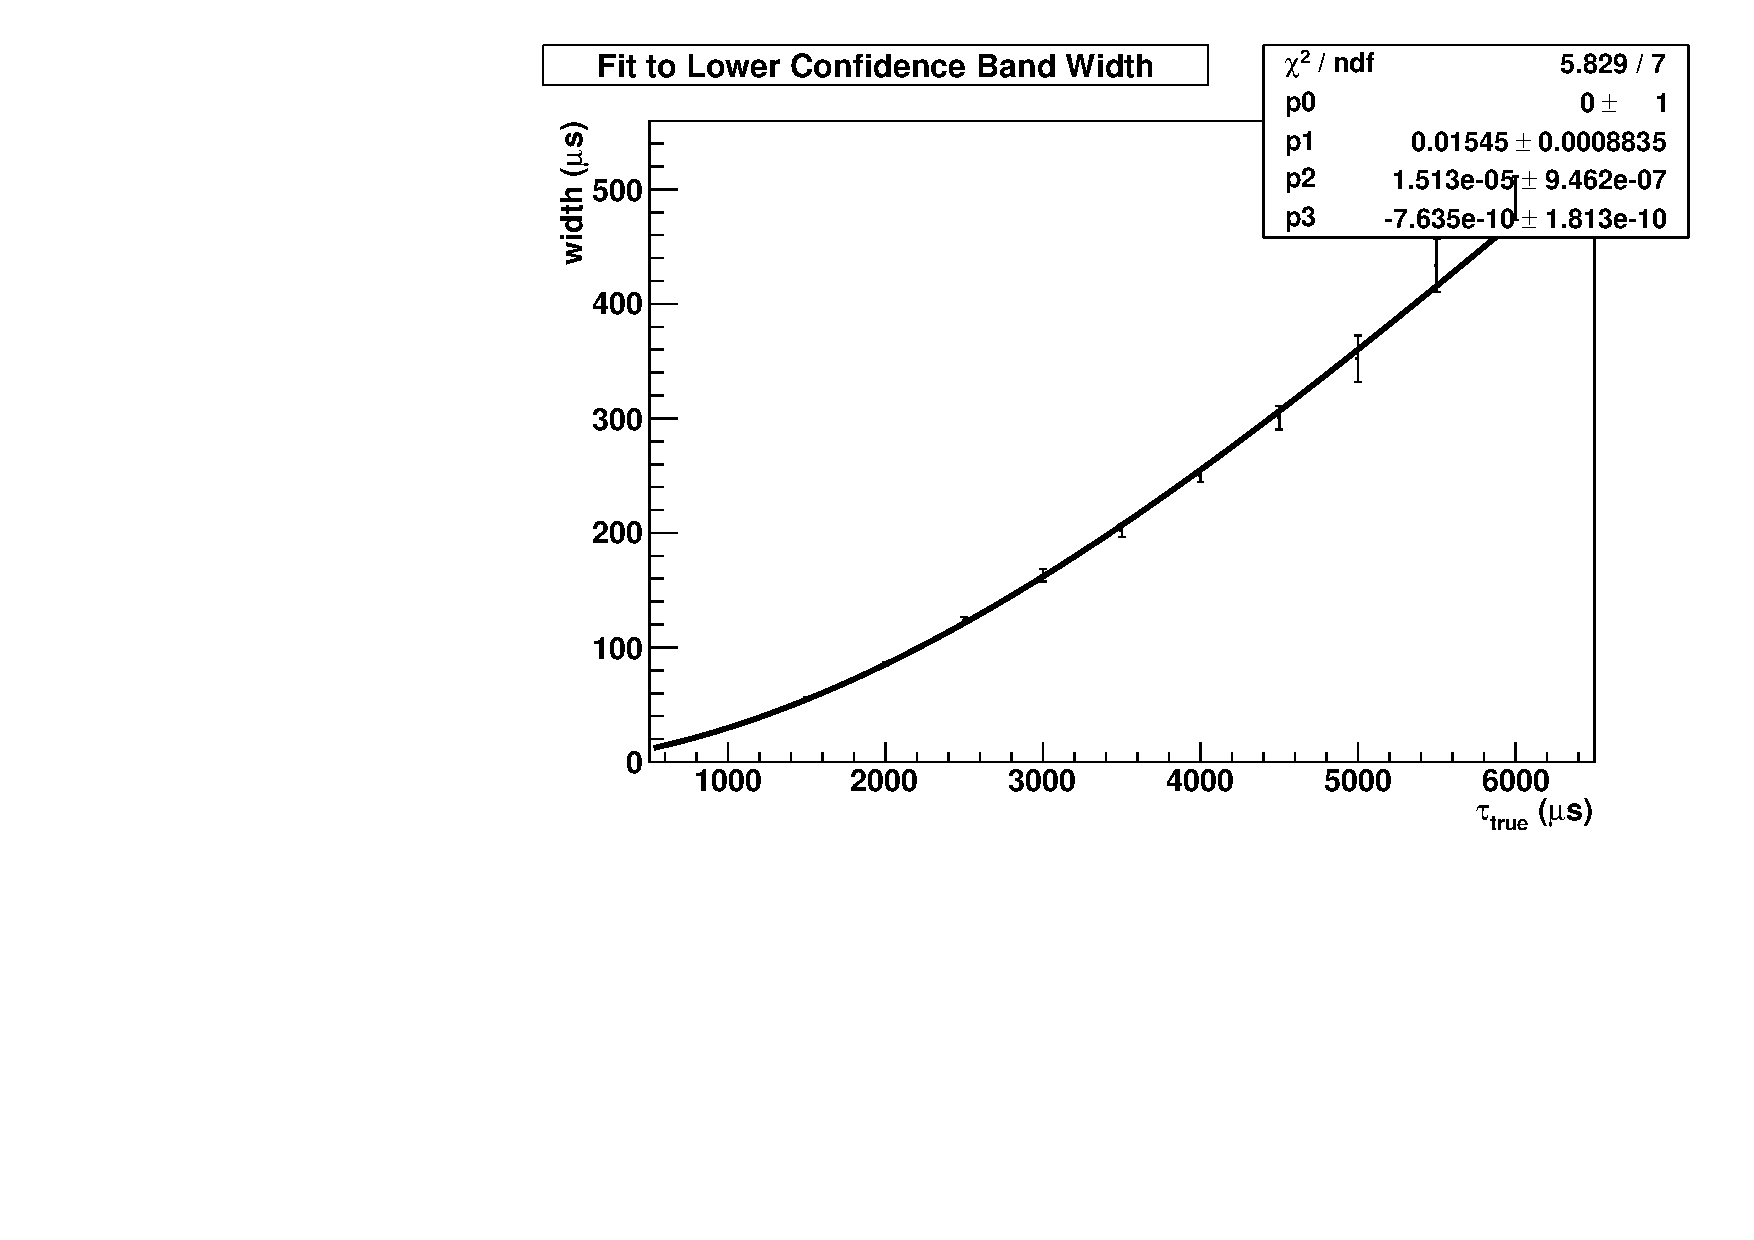
\includegraphics[width=1.0\columnwidth]{./plots/el_sim_errm_fit.pdf}
\end{subfigure}%
\begin{subfigure}[b]{0.5\linewidth}
\centering
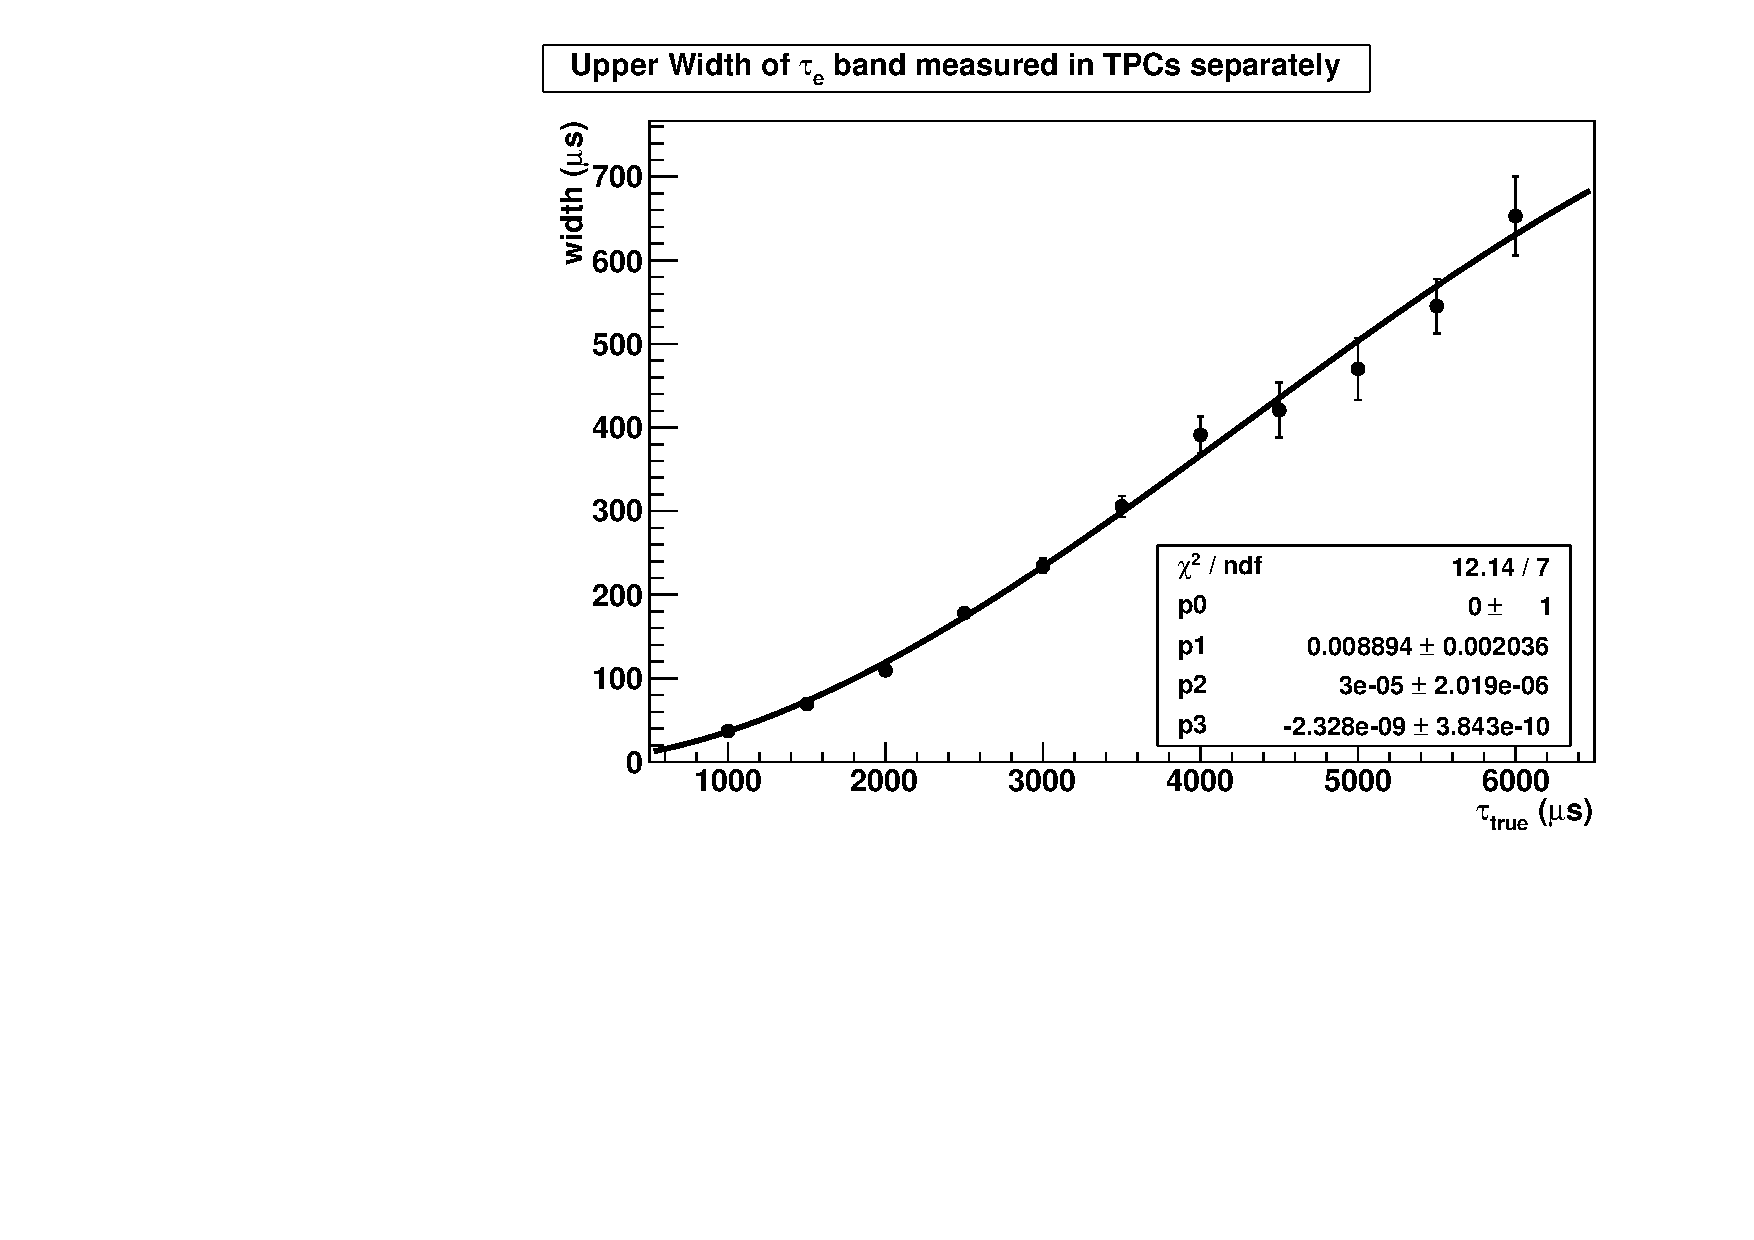
\includegraphics[width=1.0\columnwidth]{./plots/el_sim_errp_fit.pdf}
\end{subfigure}
\caption[Fits to errors on electron lifetime measurements]{The width of the uncertainty bars on single electron lifetime measurements as a function of the electron lifetime. Since the uncertainties  are asymmetric, the negative uncertainty (left) and the positive uncertainty (right) are fit separately. The fit function is a cubic polynomial.}
\label{fig:err_fits}
\end{figure}

As shown in \cref{fig:err_fits}, a polynomial function nicely fits the observed uncertainties. I tabulate the effect on electron lifetime in \cref{tab:res_dtau}. In practice, however, the effect will be smaller because a number of measurements go into the actual correction function applied to the data.

\begin{table}[htdp]
\centering
\begin{tabular}{c|c}
	\(\tau\) (\si{\micro\second})	&	\(\Delta E / E\) (\%) 	\\ \hline
	100					&	2.57				\\
	200					&	1.55				\\
	500					&	0.92				\\
	800					&	0.76				\\
	1000					&	0.70				\\
	1500					&	0.61				\\
	2000					&	0.55				\\
	2500					&	0.51				\\
	3000					&	0.47				\\
	3500					&	0.44
\end{tabular}
\caption[Electron lifetime uncertainty effect on resolution]{The effect of the electron lifetime uncertainty on energy resolution. This is based on the parameterization shown in \cref{fig:err_fits}. Note that the reported resolution assumes only one measurement is used for the correction. In practice, more measurements are used, and so the effect will be smaller.}
\label{tab:res_dtau}
\end{table}

\section{Measurements of Electron Lifetime in EXO-200}

Calibration runs taken every 1--2 days serve to measure the electron lifetime in EXO-200. In a typical calibration run, a \thorium{228} source at the cathode creates 250000 events in the TPC. Of these, approximately 2500 are single site events within 2\(\sigma\) of the full-absorption peak.

\subsection{Time Variation and Correction Function}

The measured electron lifetime varies in time. Usually, this variation is small and within the measurement error. However, events such as a feed of gas into the xenon recirculation loop (which might introduce impurities), or changes in the recirculation rate can cause more significant variation. To account for this, a piecewise polynomial is fit to the measured electron lifetimes. This piecewise polynomial can be discontinuous across sudden changes in electron lifetime. A cessation of recirculation, such as by a pump failure, can cause such a sudden change. The polynomial degree can change when the behavior of the electron lifetime changes, such as when rapidly-increasing lifetime after resuming recirculation becomes a steady-state, slowly-varying value. \Cref{fig:el_time_variation} shows the time variation and the polynomial fit for the separate TPCs. Separate electron lifetimes are used for the different TPCs because there could be some purity gradient in the chamber, and splitting the chamber in half provides a modest approximation, and because the measured values in the different TPCs sometimes vary outside of each others' confidence bands.

For a good event in EXO-200, the reconstruction algorithms find both a drift time and an (attenuated) ionization signal. The polynomial fit described above provides an estimate of the electron lifetime at the event time. \Cref{eq:exponentialtaue} provides a recipe for finding the original ionization signal from the attenuated signal, using the drift time and measured electron lifetime.

\subsection{Electron Lifetime in Low Electric Field}

\subsection{Comparison with Gas Purity Monitor Readings}

\subsection{Comparison with Pump Speeds}

\end{document}